\documentclass[10pt,twocolumn,letterpaper]{article}
\usepackage{times}
\usepackage{fullpage}
\usepackage[margin=1.0in]{geometry}                % See geometry.pdf to learn the layout options. There are lots.
%\geometry{letterpaper}                   % ... or a4paper or a5paper or ... 
%\geometry{landscape}                % Activate for for rotated page geometry
%\usepackage[parfill]{parskip}    % Activate to begin paragraphs with an empty line rather than an indent
\usepackage{graphicx}
\usepackage{amssymb}
\usepackage{epstopdf}
\usepackage{tabularx}
\usepackage{fancyvrb}
\usepackage{listings}
\DeclareGraphicsRule{.tif}{png}{.png}{`convert #1 `dirname #1`/`basename #1 .tif`.png}

\title{Who's the BOSS? Getting Buildings under Control}
%\author{Stephen Dawson-Haggerty}
\newcommand{\etc}{\textit{etc}}
\newcommand{\implname}{BOSS~}

%\date{}                                           % Activate to display a given date or no datesen

\begin{document}

\maketitle
\thispagestyle{empty}
%\section{}
%\subsection{}

\subsection{Introduction}
The United States leads the world in per-capita energy consumption.
Our electricity use has consistently increased over the last 40 years~\cite{oecd2011} and other parts of the world are rising all 
too rapidly.  With the specter of climate change and the increasing cost of energy, we must explore new
ways for individuals to gain visibility and insight into their energy consumption in order to optimize and reduce it. 
With the increasing penetration of embedded sensors in the environment and
the continued rise in smartphone adoption, we see an opportunity for smartphones to bridge the physical world
to our computational infrastructure and provide an `energy lens' on the physical world.  

We use mobile phones to construct an entity-relationship 
graph of the physical world and combine it with streaming sensor data in order to perform detailed energy-attribution.
We limit the scope of the world to a single building domain.  We have designed and implemented a real-time, mobile energy auditing
application, called the `Energy Lens', that allows us to collect information about 
things throughout the building and how they are related to each other.  For example, computer X is inside 
room Y and connected to meter Z.  Then, we use these relationships to guide our data look-up and analytical
calculations.  For example, the load curve of room Y consists of the sum of all the power traces for loads
inside room Y.  We use the mobile smartphone as the main input tool.  Our work examines \emph{three main challenges} in setting up and 
deploying a real, whole-building infrastructure to support real-time, 
fined grained energy analytics.  

The first challenge is related to tracking and mobility.
The use of mobile phones presents classical, fundamental challenges related to mobility.  Typically, mobility
refers to the phone, as the person carrying it moves from place to place.  However, in the energy-attribution
context, we are also referring to the movement of energy-consuming objects.  Tracking their relationships to spaces 
and people is as important as tracking people.  We describe how we deal with \emph{both moving people and 
moving objects} and show that these historically difficult problems can be addressed relatively easily, if the proper infrastructure is 
in place.  %We provide evidence that the approach is simple, incrementally deployable, and scalable.

The second challenge is about capturing the inter-relationship semantics and having these inform our  analytics.
We adopt the general notion of physical tags that identify objects in the world.  Our system uses \emph{QR codes} to tag things and locations 
in the physical world.  However, \emph{any tag that provides a unqiue identifier for an object could serve the same purpose}.
Once tagged, there are three types of interactions -- 
registration, linking, and scanning -- which establish important relationships.  Registration is the act of creating a virtual object 
to represent a physical one.  Linking captures the relationship between pairs of objects.  Scanning is the act of performing an item-lookup.
Each of these interactions requires a set of swiping gestures.  Linking requires two tag swipes while the other two actions
require a single tag swipe.  Internally, we maintain a \emph{entity-relationship graph (ERG)} of things, people, and locations, that gets
updated through these sets of gestures.

The third challenge is about indoor network connectivity and access.
In order to connect these components, we rely on having `ubiquitous' network connectivity.  However, in practice, network
\emph{availability} is intermittent and our system must deal with the challenges of intermittency.  We discuss how caching
and logging are used to address these challenges.  Moreover, when connectivity is re-established, we must deal with
applying updates to the ERG, as captured by the phone while disconnected.  
% Conflicts can also occur during an update.  For example, the two updates may disagree about which items are attached
% to which meters.  We implement a very simple conflict resolution scheme, described in section~\ref{sec:conflicts}.
% Finally, certain physical-state transitions are represented as a set of updates to the ERG that must be applied 
% atomically.  We implement transactions in the log-replay and transaction manager.
% Our `Energy Lens' system is deployed in a building on our campus.  We discuss
% its architecture and our design choices.  
  
% We also discuss novel strategies for tracking moving people/things and describe how we implement these in our system.  In summary, our work
% makes the following contributions:

% \begin{itemize}
% \item We design and implement a system that captures and combines physical entities, their inter-relationships, and real-time sensor data 
% 		in buildings.% using mobile phones, qr code, and a cloud-based infrastructure.
% \item We observe that certain combinations of swipes give us useful information to set the location of people and things over time.
% 		We codify this observation in our \emph{context-tracker} and use it to maintain consistency between the entity-relationship graph and the 
% 		state of the physical world.  To the best of our knowledge, this is radically different from the approaches in standard 
% 		localization techniques.  However, we argue that it can be used to \emph{enhance} their accuracy and overall performance.
% \item We implement a prefetching algorithm to obtain context-dependent information to both improve performance and
% 		enable disconnected operation.  We also design and implement a log-replay and transaction manager over our data management layer.  We describe how different conflict-resolution policies can be implemented and our rationale for the policies we chose.
% \end{itemize}

% \vspace{0.08in}

% In the next sections we go through a motivating scenario.  We then discuss some related work, followed 
% by the system architecture, evaluation, and future directions.

\section{Background and Motivation}

% Existing system architecture for buildings is rooted in past practice, and does not look forward to a networked future.

\subsection{Existing Building Systems}

A large modern commercial or industrial facility represents the work of thousands of individuals and tens or hundreds of millions of dollars of investment.  Most of these buildings contain extensive internal systems to manufacture a comfortable indoor environment: to provide thermal comfort (heating and cooling), a good air quality (ventilation), and sufficient lighting.  Other systems provide for life safety with fire alarms and security, and the design of a particular building takes into account many other considerations.  All of the active components of the system typically require management interfaces, just like components in a computer system.  System managers need the ability to troubleshoot problems, adjust schedules, and change set points. 

This control in existing building systems operates on two levels.  Direct control is performed in open and closed control loops between sensors and actuators.  In a direct control loop, a piece of logic examines a set of input values, and computes a control decision which directly commands an actuator.   These direct control loops frequently also have configuration parameters which govern their operation; these are known as set points and are be set by the building operator, installer, or engineer.  Adjusting set points and schedules forms an outer logical loop, known as supervisory control.  This logical distinction between types of control is frequently reflected physically in the components and networking elements making up the system: direct control is performed by embedded devices called Programmable Logic Controllers (PLCs), which are directly connected to the sensors and actuators, while supervisory control is managed over a shared bus between the PLCs.  This architecture is logical for implementing direct control loops since it minimizes the number of pieces of equipment and network links information must traverse to affect a particular control policy, making the system more robust.  One property of this system is that interaction with the outside world is achieved through the changing of set points (and less frequently, control logic), over the supervisory control bus.  

Figure: control system physical/logical architecture

Figure: HVAC loop with VAVs, chiller, 

% Something about lighting and HVAC.

%However, it is highly desirable to integrate additional information into these control loops.  A simple addition of weather forecasts can make a huge difference in the efficiency with which a building operates, since it allows the system to take advantage of unexpectedly favorable conditions or otherwise adapt to changing climatic conditions.  However, adding new information must be done carefully, with an eye to preserving system qualities such as robustness, simplicity, and predictability.
%
%\subsection{Instrumentation heterogeneity}

%Existing building systems typically have one o
\subsection{Motivating Applications}

The need for a new operating system for the building is motivated by several concrete applications we wished to deploy on our building.  Applications developed for the built environment range from fine-grained energy accounting to localized climate control.  Some of them require input from the occupants; data from sensors attached to personal items and control signals initiated by occupants.  While others require no direct occupant participation.  For example, control applications that override local control loops to maximize energy efficiency while maintaining occupant comfort.  We also wish to support dashboard applications that gives occupants and the building manager a global view of building performance, or analysis applications that run outside the built environment to analyze the operational performance of the building, feed performance forecasting models or combine building sensor data with external signals, such as weather and energy pricing.

Although versions of these applications can be deployed directly using existing systems, developing them requires low-level knowledge about the construction of a building, restricting their generality. It also requires careful reasoning in each case about the effect of various types of networking and system failures.  Moreover, one needs to consider issues of privacy and controlled access to data and actuators, and more broadly provide mechanisms that provide isolation and fault tolerance in an environment where there may be many applications running on the same physical resources. Experience with ad-hoc development of this style of application led us to the conclusion that better abstractions and shared services would admit both faster and easier application development, as well as more consistent and robust fault tolerance.

The first motivating application is a {\it temperature float} application.  Ordinarily, temperatures within a zone is controlled to within a small number of degrees Celcius.  This drive for reaching an exact setpoint is actually quite inefficient, because it means that nearly every zone is heating or cooling at all times.  A more relaxed strategy would be one of {\it floating}: not attempting to effect the temperature of the room when it is within a relative wide band; however this is not one of the control policies available in typical commercial systems.  

A second application was developed as part of a program to improve efficiency and comfort by giving occupants direct control of their spaces.  Using a smart-phone interface, occupants are able to directly control the lighting and HVAC systems in their spaces; a social component resolves conflicting preferences between neighboring occupants.  The application requires the ability to command the lights and dampers in the space to, for instance, guarantee that the lights are on for a period of time and to deliver services like a ``blast'' of hot or cold air to address temperature or ventilation complaints.

A third application is an energy audit and live energy viewer of the building.  Using a smart-phone interface, occupants input information about the structure of the building and the relationship between sensors and devices.  This requires access to a uniform naming structure and streaming sensor data coming from physically-placed sensors.  The former to capture the inter-relationships between building locations, sensors, and loads (energy consumers) and the latter to provide up-to-date information about physical measurements taken in locations throughout the building.  For example, an occupant may wish to see the total energy consumed by all plug-loads on a particular floor.

Our final application is an offline analysis tool for characterizing data streams and finding if the semantic information, as captured by the naming structure mentioned above, is accurate.  This application requires access to the uniform naming structure and assocaited historical sensor data.

\subsubsection{Architectural implications}

The \emph{temperature float} application highlights the need for attaining feeds in real-time and locating the appropriate setpoint actuator for each temperature control unit.  The architecture must treat streaming data natively, providing mechanisms for subscribing to incoming feeds.  It must also provide a way to actuate devices explicitly.  Furthermore, contextual metadata should be in place so that application can determine which devices it is receiving data from and which device it is actuating.

The \emph{mobile climate control} application highlights the need for leasing control to the HVAC components and lighting fixtures.  Access control is a concern here.  The ``lease'' is a useful mechanism for providing \emph{temporal isolation}.  A system must include a mechanism that allows application to temporarily own resources and forcibly reclaim those resources if necessary.

The \emph{audit} application highlights the need to couple semantic information with streaming sensor data in a uniform fashion and a way to meaningfully combine it with raw sensor data.  Our system should provide a mechanism that allows users to leverage this structure when possible without constraining them if the structure needs to change over time.  It also emphasizes the need for real-time data cleaning and aggregation.  Sensor feeds are quite dirty, often containing errant or missing values.  Security and privacy play a factor here as well.  This application makes use of personal data quite explicitly this motivates the need for a way that applications and users can control who can access their personal feeds.

The \emph{analysis} application highlights the need for generic interface for ease of integration with external tools.  The filesystem presents the deployment as a distributed filesystem and allows users to seamlessly interact with and query their environment without having to write tools to integrate with their local application.  In order to allow a broader range of applications, especially those that involve analysis rather than direct application building, our system must have multiple interfaces for access deployment information and sensor data.

%
%\subsection{Challenges for BOSS Design}

%\begin{itemize}
%\item security
%\item consistency
%\item reliability
%\item isolation
%\item scheduling
%\item naming
%\item hardware abstraction
%\end{itemize}
\section{Design}

% + Simplify application development and support many simulatenously running apps
% 	+ provide \emph{shared services} and \emph{controlled access} to underlying sensors, actuators
% 	+ maintain \emph{isolation} while allowing \emph{explicit sharing} between applications (protection)
% 	+ provide a uniform, common namespace to build applications on 
% 	+ improve programability while maintaining robustness (fault tolerance)

We propose a new architecture for building systems where the main goal is to {\bf ease application development and support many simulatenously running applications}.  More specifically we look to:

\begin{itemize}
\item improve programmabilty through useful \emph{abstractions} for application developers.
\item provide \emph{shared services} and \emph{controlled access} to underlying sensors, actuators.
\item maintain \emph{isolation} and \emph{protection} while allowing \emph{explicit sharing} between applications.
\item maintain robustness and \emph{fault tolerance} for running applications and resources.
\end{itemize}

Our architecture consists of three layers, the hardware-abstraction and control-transaction layer, the naming and data-access layer, and the application layer.  A high-level view of each layer and its constituents is shown in Figure~\ref{fig:arch-layered}.  In layer 1, the {\bf hardware abstraction layer} consists of a hierarchical set of interfaces which provide interfaces to the underlying physical building hardware at increasingly abstract levels.  The {\bf transaction} interface is the run-time abstraction responsible for implementing command decisions made by applications.  In layer 2, we provide a rich {\bf application runtime} for creating reliable software on top of a building, which includes a global {\it namespace} provided by the directory service, and time-series service for accessing and cleaning historical data.  

For applications that require a more structured, uniform namespace we provide a filesystem interface over the directory and time-series service.  The filesystem allows users to interact with building sensors through read/write file operations.  The fileystem also provides a level of {\it security} while performing file operations and sharing data with other applications; users are provided with a unique identifier and associated permissions that allow them to view and share files among and across applications.

\begin{figure}[htb]
\centering
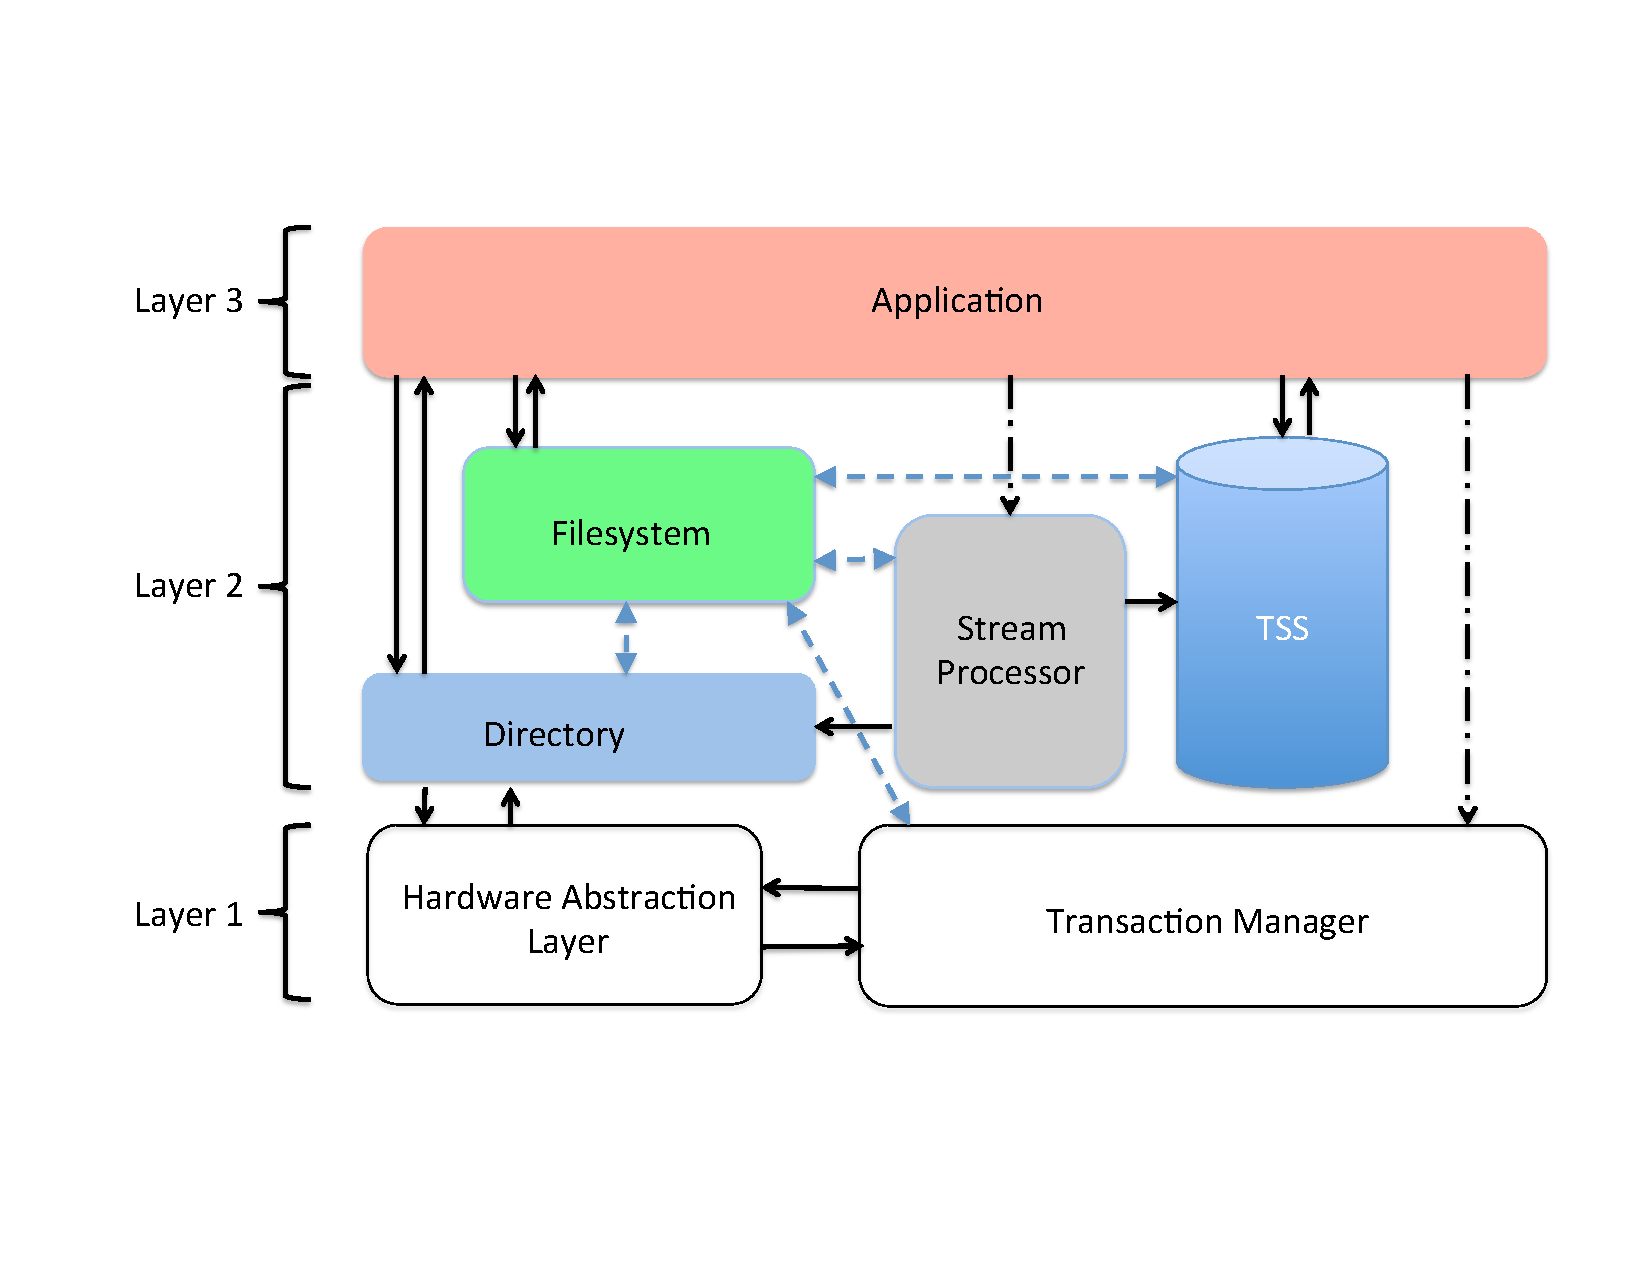
\includegraphics[width=\columnwidth]{figs/arch-layered}
\caption{System architecture.  Layer 1 consist of the hardware abstraction (HAL) and control-transaction components.  Layer 2 consists of components for naming and data access.  Layer 3 is the application layer.  The application layer can access
any of the underlying components directly, except the HAL.}
\label{fig:arch-layered}
\end{figure}

Finally, layer 3 consists of applications for the built environment.  The underlying architecture should support multiple applications running simultaneously on the underlying infrastructure.  Some may consist of {\bf control processes} that represent existing control strategies.  Robust control processes require support for wrapping applications to allow them to be dynamically migrated by the system, and mediated access to other required functionality.

% With the goal of improving programability while maintaining robustness, we propose a new architecture for building systems; shown in Figure \ref{fig:arch}.  This architecture consists of four interlocking layers.  The {\bf hardware abstraction layer} consists of a hierarchical  set of interfaces which provide interfaces to the underlying physical building hardware at increasingly abstract levels.  Secondly, we provide a rich {\bf application runtime} for creating reliable software on top of a building, which includes a global {\it namespace} provided by the directory service, and time-series service for accessing and cleaning historical data.  Finally, the {\bf transaction} interface is the run-time abstraction responsible for implementing command decisions made by applications.  We have chosen a transactional metaphor for this interface, because it is required to provide isolation between concurrent control inputs; scheduling between different applications; and fault tolerance (at least across fault domains).
% Finally, {\bf control processes} implement the logic of the system and may represent existing control strategies, or novel new applications.  Robust control processes require support  for wrapping applications to allow them to be dynamically migrated by the system, and mediated access to other required functionality.

% \begin{figure}[htb]
% \centering
% 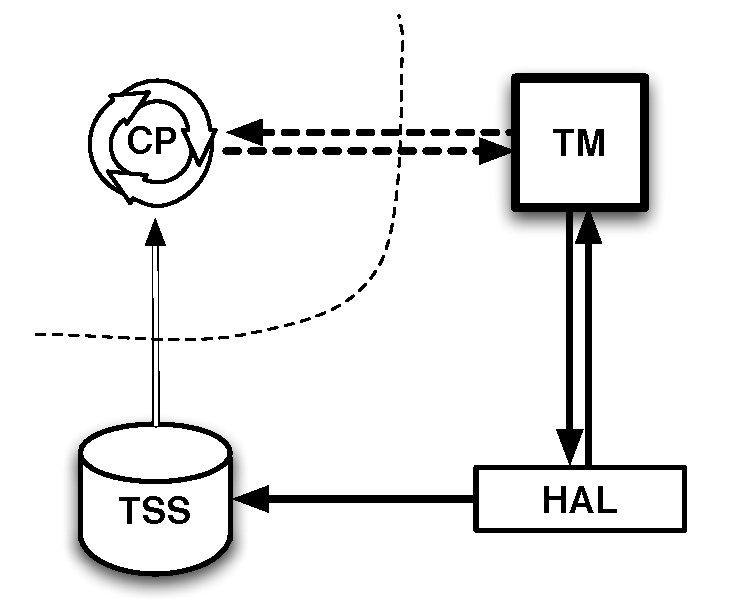
\includegraphics[width=\columnwidth]{figs/comm}
% \caption{System architecture.  Key components are the hardware abstraction layer (HAL), control processes (CP), Transaction Managers (TM), and time-series server (TSS).  Communication within a fault domain is unrestricted, but all control inputs must be mediated by a Transaction Manager (TM), located in the appropriate domain.}
% \label{fig:arch}
% \end{figure}

\begin{table*}[htb]
\centering
\begin{tabularx}{\textwidth}{|l|X|X|}
\hline
Architectural component & Function & Placement \\
\hline
\hline
Hardware presentation layer & Make the primitive low-level operations of the hardware available using a common set of interfaces. & As close to the physical sensors as possible; ideally, co-located with the transducer.\\ 

Hardware abstraction layer & Map the low-level functions of the physical hardware into multiple higher level abstractions.  & Anywhere; should be persistent.\\

Directory & Place devices from the HPL and HAL into a namespace. & Replicated; may be offsite.\\

Historian & Maintain a history of readings from the sensors and actuators. & Replicated; may be offsite. \\

Filesystem & Provides explicit structure to the underlying namespace. & Replicated; may be offsite. \\

Transaction manager & Provide ``all or nothing'' semantics when applying control inputs; schedule conflicting and concurrent commands.  & In the same failure domain as the HAL used to affect the changes. \\

\hline
\end{tabularx}
\caption{Description of architectural components}
\end{table*}

% How does discovery work? What is the namespace? 
%
%\subsection{Fault domains}

%Execution in this architecture is distributed across three conceptual domains: the lowest, the sensor and actuator plane, building-level controllers, and Internet services.  The purpose of distinguishing these domains is not because of a difference in capability (although there are surely huge differences), but rather because we wish to allow these to be reasoned about in terms of the implications of a failure; we call them ``failure domains.''  For instance, a failure of the network connecting a floor-level panel to other building controls does not compromise that panel's ability to actuate based on the directly-connected inputs and outputs, but it does prevent it from contacting an Internet service for instructions on what to do.  The tolerance of a particular control loop to failures can be determined by examining which data are needed as inputs, and from which tiers they originate.  
%This model could be generalized to extend to an arbitrary number of domains, but we will carry thorough our analysis with this simple example.

\subsection{Hardware Abstraction Layer}

One function of traditional computer operating systems is to provide a convenient abstractions of physical resources.  The interface to hardware devices is low-level and heterogeneous in both computer systems and in building systems.  At the lowest level of the hardware interface stack is a Hardware Presentation Layer (HPL).  The HPL hides the complexity and diversity of the underlying communications protocols and presents hardware capabilities through a uniform, self-describing interface.  The HPL abstracts all sensing and actuation by mapping each individual sensor or actuator into a {\it point}: for instance, the temperature readings from a thermostat would be one sense point, while the damper position in a duct would be represented by an actuation point.  The HPL provides a consistent method of collecting data from the sensors and commanding individual actuators.
The layer also provides the basis of naming in this system: each sense or actuation point is named with a single, globally unique identifier.  This functionality is distributed across the computing resources closest to each sensor and actuator; ideally it is implemented natively by each device.


%We develop a distributed HPL which abstracts the numerous vendor-provided interfaces for retrieving data and effecting commands into a simple RESTful interface.  The HPL is distributed because the sense and control points are themselves distributed throughout the physical environment.  It is desirable to place the HPL for each piece of hardware as close, physically and topologically, to the device as possible.
 
On top of HPL we form a Hardware Abstraction Layer.  The task of this layer is to provide the basis for mapping  underlying primitive hardware operations into useful higher-level relationships.  As in computer systems, it is often desirable to access the same physical hardware using multiple abstractions.  For instance, multiple network-layer protocols are run on top of the same physical network interface.  The corollary for the built environment is that multiple views of the same physical sensor and actuator points are possible.  For instance, answering the question of which sense points are in a particular room has no particular relationship to which systems: lighting, climate, security, that these sense points are part of. The HAL is responsible for representing the various types of metadata about the sense and actuation points.

In order to represent the relationships between sensors and actuators, the HAL uses key-value {\it tags} which can be applied to each sense and actuation point.  By using tags, we avoid the need for imposing a schema on the metadata to be provided, allow representation of both hierarchical and subset relations, and support mapping multiple ontologies onto these points.  These tags can be applied directly at the device itself, or within the global namespace formed by the directory.  This is important, because some of this information such as the type of instrument present, and its sensing modalities are natural to apply at the point of instrumentation, while other information like the relationship of an actuator to other system components are only known later, once a global view of the system has been established.

A HAL from a physical system differs from that for a computer system in several ways.  A major difference is that in a computer system, the ``virtual'' representation of the system (made up of the device drive state, \etc) contains essentially everything relevant about the state of the underlying physical system.  In the physical environment, the virtual representation is unlikely to be nearly as complete; the underlying physical system has complicated physical dynamics which is it extremely rare and difficult to fully capture.  Therefore, we have much less observability and control over how actions made on the virtual representation will impact the physical system and the observable quantities.  Furthermore, in a computer system the types of hardware are known ahead of time: the architecture of all computers falls essentially into one of several models of bus interconnections of the various components.  In contrast, although the individual components of building systems are relatively standardized, the relationships between them depend on the design of a particular building.    For instance, many buildings have similar systems for providing cooling: air is blown through ducts, where it is cooled and ultimately distributed into spaces through variable air-volume (VAV) boxes.  However, the behavior of this system depends heavily on the routing of the network of ducts and placement of VAV boxes, which is customized for each individual building.


%Ultimately it is desirable that advanced building modeling and control be possible without manual setup, operating on computer-readable descriptions of the spaces and systems, and sensor data as input and outputting optimized parameters. Human intervention should only be required in order to specify comfort and safety requirement.  However, a key problem in achieving this is discovering the relationships between the data streams and the physical environments they interact with.  Ample descriptions of these relationships are already available in the form of architectural and engineering drawings of various spaces and systems, Building Information Models (BIM) which have been assembled as part of construction, renovation, or retrofitting, energy models such as those processed by Energy+ or DOE2 simulators, and operator screens presented by existing control systems.  However, this data also must be cleaned and validated in order to be useful, since the drawings may not always reflect as-built construction, and the BIM data could represent a concept that was subsequently scaled back.  It also often does not contain a complete representation of the installation building systems.  We have begun developing tools that can automatically process and extract information from architectural drawings, existing control systems screens, and other graphical representations of the building and produce computer representations of the spaces and systems therein through the use of OCR and other computer graphics techniques.  We have also begun importing, simplifying, and extracting from industry-standard BIM formats like IFC models of physical spaces, in order to extract the relevant metadata.

% HAL

\subsection{Directory}

% key ideas: global search/namespace for poitns

The HAL provides distributed real-time access to the system under control; however, implementing control strategies and applications requires a global view of the system and access to stored data.  The directory provides a {\bf global view} of this metadata.
%
The sensor and actuation points identified by the HPL are objects in the namespace of the system; because this information is distributed across all of the sensors and actuators, it is necessary to have an operating system component which allows applications to query it in a straightforward way.
%
The directory service allows applications to locate sense and actuation points by performing queries on the key-value metadata.  It is often desirable to query across multiple ontologies at the same time; for instance, ``locate the power reading (measured in kW) for the air conditioning component servicing a particular room.''  This requires accessing at least three separate mappings: the instrument mapping, recording information about the instrument, the spatial mapping locating that room, and the systems mapping that room to the system providing service.

The directory can be thought of as an analog of the standard unix {\tt /dev} namespace which has been redesigned around database filesystem principles.  The {\tt /dev} tree is typically organized to match the underlying system architecture of the computer system; for instance, {\tt /dev/bus/usb/001} contains devices on the system's first USB bus.  Building systems have an analogous structure corresponding to the topology of the building network, which specifies which PLCs and head-end nodes the sensors is accessed through.  
% Because this topology does not map neatly onto any more useful representation such as where the devices are in space or which system they are part of, it is difficult to explore.  

\subsection{Filesystem}
For a certain class of applications we wish to support, files are the least common denominator for accessing sensor information.  Many services on sensor data can be provided through the filesystem interface.  Allowing applications to read/write files to interact the building is an effective approach for supporting legacy client applications.  For example, applications written in Matlab or R would not require any integration code to fetch sensor data; only local file reads/writes are necessary to attain the necessary data for analysis.

The filesystem interface provides a structured version of the directory service and provides a direct way to express structured semantic information and couple it with sensor/actuator information.  For example, spatial relationships are inherently hierarchical.  Buildings have floors, floors have rooms, room have sub-spaces.  Sensors can be placed within the spatial namespace in order to encode the relationship between sensors and spaces explicitly and can be accessed via the associated spatial path (i.e. {\tt /building/floor4/410/temp/reading}).  Moreoever, the use of symbolic links allows users to create separated sub-trees that capture other hierarchical relationships, such as aggregation groups.  The HVAC system has no clear hierarchical relationship, but the components of it do.  The HVAC system consists of vents, ac units, heaters, pumps, valves, etc.  Each of these components also have sensors attached.  Therefore it can be constructed in a similar fashion as the spatial namespace.  \emph{Aggregation groups can guide namespace construction when there is no clear structural hierarchy in the physical system}.  Moreover, symbolic links allow for sensor access to be referred to through mutliple names.

Security and access control can be taken directly from the Unix filesystem security model.  Files that represent physical and logical resources are owned and shared by the user that created them.  Each application sees a different view of the files in the system and can share access by giving read/write/execute rights to other users, as identified by their {\tt username}.

% Although an actual hierarchical structure for the naming scheme in a building is an open question, we found applications settling on a structure that groups components in the building as constiuents of an aggregate.  We also found hierarchies guided by spatial relationships.  These and others should be supported and interpretted by individual applications and supported by the filesystem.

Since we are fundamentally dealing with streaming data, the filesystem should provide access-to and management-of stream processing facilities.  This can be achieved through overloaded Unix filesystem  mechanisms.  For example, the use of ``pipes'' can accomplish the goal of re-direction and data-flow declaration.  Applications should be able to pipe streaming data through local processing scripts as well.  Actuators can also be represented as a file, where reads fetch the current state and writes change the state of the actuator.

\subsection{Historian}
The historian provides access to historical data, frequently needed for analysis.  The data model is relatively simple: there are a large number of time-series generated by the sensors and actuators; a time series is simply a set of related {\tt (timestamp, value)} pairs which we call {\it readings}. 
%
Typical access patterns for historical data have characteristics somewhat different than those traditional relational databases are optimized for.  Data are typically accessed by performing range-queries over time stamps and streams; for instance a typical query might extract all room light-level readings for a period of one month.  Even a modest-sized installation will easily have tens of billions of readings stored and even simple queries have the potential to touch hundreds of points.  New data is nearly always gradually appended to the end of the time series, because the data comes from individual measurements taken by the sensors and published by the HPL.

Finally, it is impractical to keep the highest-resolution data from all sensors forever since the value which can be extracted from this old data frequently can't justify the cost of maintaining the history; therefore the historian must have the facility for degrading or compressing older data.

%Performing these operations efficiently is the task of the archiver.  The archiver forms the application interface for retrieving stored data.  Its design consists of two parts: a stream selection language, and a data transformation language.  Using the stream selection language, applications can inspect and retrieve meta-data about the different time-series in the stream.  The data-transformation language allows clients to apply a pipeline of operators to the retrieved data to perform common data-cleaning operations.  This both moves complex processing logic out of the applications, allowing them to focus on making the best use of the data, and also enables the possibility of optimizing common access patterns.  For instance, if the sensor data is generated by an instrument every 5 seconds, but only accessed after subsampling to 5 minute resolution, the system may materialize a 5-minute view of the data to avoid loading the source data for each request.

\subsection{Stream processor}
Before stored data can be used, it must typically be {\bf processed and cleaned} since raw sensor data is quite dirty; for instance, timestamps need to aligned and the data may be resampled and smoothed.  Furthermore, since real-time data is important, especially for control applications, there is a clear need to process and clean the data in real time.  A stream processing element is an important service that must be included in the archiecture.  The engine should not only help manipulate individual data points, but should optimize for operating on vectors of data points.  Most of the oeprations for data cleaning are performed on data vectors, the same should be provided here as well.

% The main principal is the user/application, as identified by a username and {\tt uuid}.  Each {\tt uuid} is coupled with file access writes for each file that they own or have certain access to.  Sharing can be done explicitly by specifying the username, file, and operations you want to add or remove for users to the files you own.

% It couples semantic information and sensor data and lays it out hierarchically.  For example, a spatial hierarchy is constructed as a set of directories with each containing the sensors within it.  This filesystem, however, makes use of special files to incorporate access to stream data.  Sensor data streams are represented by special files that can be ``tailed'' to see the incoming stream.  Moreover, streams can be piped through local or remote locations by using a standard unix pipe command.

% The filesystem provides security mechanisms and access modes familiar to typical Unix applications; interaction with the deployment happens through local file reads and writes.  The filesystem layer assigns a unique id to a each user or application.  Access rights are associated each unique identifier -- a simplified access control list approach similar to unix.  Writing to a special ``stream'' file issues a query to the associated time-series service that contains the time-series data.  In that way applications can read the file after it is written to and load to data for local processing.

% Built with streaming data in mind, the filesystem also supports stream process management.  A class of special files called ``processors'' can have data piped through them for analysis and managed through the filesystem.  In addition, it supports the ability to aggregate data of the same ``units'' and makes the output accessible the filesystem as well.  Application-specific naming conventions have come about from using the use of this feature.  The guiding principle is to contain all associates data streams in directories as you would like to aggregate them by.  For example, all HVAC components go in the {\tt /building/HVAC} directory so that you may query this directory for aggregate HVAC information, such as total energy consumed by the HVAC system.

\subsection{Control transactions (CTX)}

It is desirable that control policies be extended or modified across multiple failure domains for a multitude of reasons.  Internet-based services may have more processing and storage than is available in the building, or may wish to implement proprietary logic.  It may also be simpler and more concise to express the desired outcome in terms of a set of changes to be made than to program the underlying controllers individually; ideally changes would be expressed in terms of desired outcome (make this room warmer) rather than the detailed implementation (increase the set point, re-set the chilled water temperature, and slow down the cooling loop pumps).  However there are real problems with performing automatic direct or supervisory control over the Internet or building network.  For direct control, latency may be an issue.  There can be concurrency issues when changes are made by multiple parties.  A failure of one  domain can leave the system in an uncertain state.

In order to help resolve these issues, we propose using an extended {\it transaction} metaphor for affecting changes to control state.  Transactions in database systems are a way of reasoning about the guarantees made when modifying the data.  In a control system, a transaction is a similar way of reasoning about what happens when sequences of control inputs are made by different parties.

Control transactions operate conceptually at the supervisory level; but we expose a significantly richer interface than simple set-point adjustment.  Most basically, a control transaction may write new values to a set of actuators, or update parameters being used by direct control loops; for instance, command the lights to turn on or change a term in a PID controller.  Generally, a transaction may replace the direct control logic with a new piece of logic; for instance, replace a PID loop with a new loop.  In addition to the action to be performed, a control transaction consists of several other concepts.  One is a {\it lease time} during which the control action is to be valid, or the new loop active.  When the lease expires, the transaction manager will execute a separate ``END'' block of the transaction and then restores control of the system to the next scheduled direct controller.  

\begin{itemize}
\item {\bf Concurrency Isolation}: Traditional database systems inform the user what view of the data he will see, when there are multiple writers are present.  The typical choice is to provide strong {\it isolation} between multiple accessing processes.  In a control system, isolation takes on a different meaning because control taken on one set of actuators could effect the outputs of other actuators and sensors.  We will define several senses in which transactions may be ``isolated'' while commanding a system.
\item {\bf Scheduler}: Transaction scheduling goes hand-in-hand with concurrency; each transaction is, ultimately, a set of small changes which must be applied to the system.  These must be scheduled in some way, respecting the concurrency constraints of an underlying hardware as well as the impact one set of actions will have on other running transactions.
\item {\bf Abort}: Running database transactions can be aborted when required due to a transient failure, a deadlock, or user command.  In a control system, there may be other causes.  A higher-priority transaction may require access to a resource currently used by a lower-priority transaction, or one of a set of changes may fail, requiring processing on the transaction to be aborted.  Unlike database transaction, the control transaction manager may not have control of the underlying data; for instance, there is no way to ``lock'' the value output by a sensor; it crossing a value could necessitate aborting a control sequence.
\item {\bf Rollback}: Reverting a database transaction typically involves only throwing away changes which have yet to be committed; or not writing a commit record.  Reverting a sequence of control decisions may be possible in some cases; for instance, going back to an earlier set point.  Generally, control outcomes are frequently ``path dependent''; it's never possible to revert the physical state of the world but it is possible to shift to other control strategies. 
\end{itemize}

\subsubsection{Isolation}

The notion of how two sets of control inputs can be isolated from each other in a control system is considerably more broad than that available in a database system, because transactions may interact through the physical environment.  Transactions may take complex actions which interact in physical space and occur at different levels of abstraction.

\begin{enumerate}
\item {\bf Actuator} isolation refers to isolation between the physical actuation points being accessed in the transaction.  Different transactions which are concurrent and access any of the same control points are considered to be in conflict.
\item {\bf System} isolation uses hierarchical locking to guarantee that when a control input is made, no other control input is made to the same system that would cause a conflicting result in physical space.  For instance, consider a room with two lighting systems: it should not be possible for two concurrent transactions to actuate them simultaneously.
\item {\bf Model-based} isolation is the most advanced type of isolation, at attempts to reason about isolation in terms of the effect of an action.  For instance, a transaction which increased the light level in a section of a room might or might not conflict with a second concurrent transaction which increased the light in a separate part of the same room, depending on a model of light propagation in that room.
\end{enumerate}

\subsubsection{Security and Authorization}

The transaction manager is also the logical point at which to enforce a security policy, controlling which principals can perform which control inputs\dots

The filesystem handle sceurity separately\dots


\subsection{Control processes}

The goal of this architecture is to enable the development of novel control strategies for CPS's in the built environment which use model-predictive control, occupant feedback, and many other innovative policies and then implement them in the real-world rather than leave them confined to either the research setting or proprietary, vertically integrated solutions.  Collectively, we call the software implementing these new strategies ``control processes,'' although this name belies the potential complexity in this layer.  Essentially, control processes use the interfaces presented by the Transaction Manager and the Archiver to implement control logic; we make no particular requirements about the architecture of the CP's themselves.  Equally possible CPs are a MATLAB script which subscribes to real-time data and submits control inputs based on a model, or a Ruby-on-Rails application which communicates with occupants and uses their input to make decisions.

Because of the careful design of transactions and the archiver, many of these new applications can be developed without the stringent reliability requirements traditionally required of control logic.  Furthermore, they have fewer restraints on where they can be placed in the computing infrastructure, because if they fail or become partitioned from the actuator they control, the transaction manager will simply ``roll back'' their changes and revert to a different CP which has not experienced partition or failure.

\section{Evaluation}
\label{sec:eval}
In this section we measure prefetch download times and discuss strategies for providing scalability.  We also
look at the transaction manager and evaluate conflict resolution times.

% \begin{figure}[htb!]
% \begin{center}
% 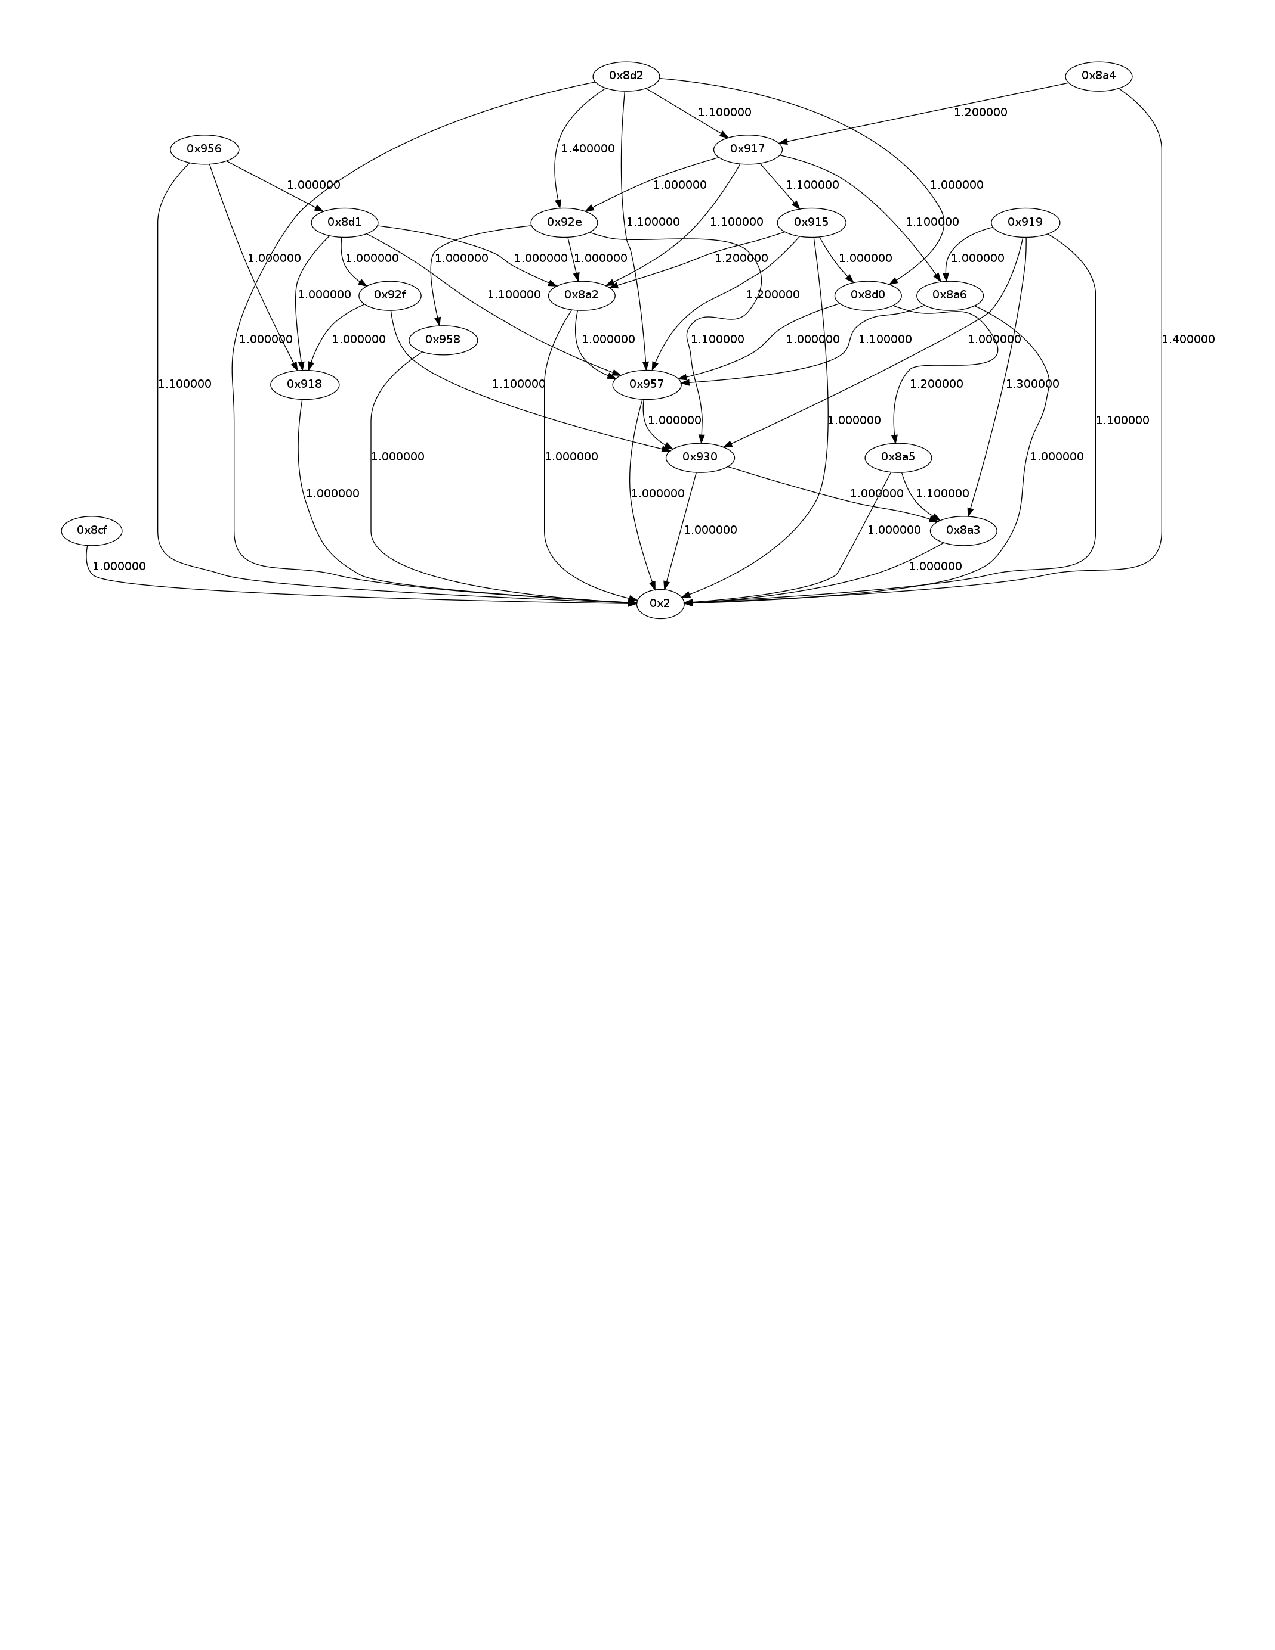
\includegraphics[scale=0.4]{figs/acmenetwork_SDH_4F}
% \caption{}
% \label{fig:acmenetwork_SDH_4F}
% \end{center}
% \end{figure}


\subsection{Prefetching}
Prefetching occurs when a user enters a new floors, as detected by a floor scan or an item
scan.  Table~\ref{tab:prefetchtimes} shows that the prefetch times scale linearly with the number of
items (and data) to prefetch.  Each node holds approximate 100 bytes or information and for
a 20-node deployment of power meters, producing 100 bytes of data per stream (3) every 20 seconds, we fetch 
approximately 1 MB of data.

These prefetch times are non-trivial to deal with, especially since they cause the phone application to slow down
until the data received and loaded into the local cache.  The overhead is dominated by the query in StreamFS that 
constructs the entire sub graph to send to the application.  For future work,  we are will implement a
callback facility and pass the application a reference to it.  The app can then periodically check back until
the query completes and the data is ready to be downloaded.  We can also include partial responses to the query
in the prefetch loop response.  This also allows user to continue using the application without any frustrating waits.

% \subsection{Log dump measurements}
\begin{table}
\begin{center}
  \begin{tabular}{| r | c  c | }
    \hline
    {\bf No. nodes } & {\bf Fetch time (sec) } & {\bf Std. Error (sec)} \\ \hline
    1 & 0.8902 & 0.0756 \\ \hline
    10 & 5.7342 & 1.7087 \\ \hline
    100 & 52.3145 & 14.1146 \\ 
    \hline
  \end{tabular}
\caption{Shows the time to fetch nodes based on the size of the fetch.  The fetch time
increased linearly with the number of nodes.  Caching maintain fetch time near
that of fetching a single node.  A callback is used when cache is invalidated.}
\label{tab:prefetchtimes}
\end{center}
\end{table}


\subsection{Log replay latency}
Table~\ref{tab:optimes} shows the  operation that the transaction manager calls on the StreamFS server.
Log replay and transaction processing is entirely dependent on the time to execute these operations on StreamFS.
There are two types of transactions, a \emph{move}, a \emph{un/bind}, \emph{un/attach}.  A move is a combination
of a `delete' and a `create link', a bind is a `create link' and an `update tags', an unbind and unattach is a
`delete' and `undate tag'.  The transaction latency is the sum of these operations.  By far the most expensive
operation is a `create node' operation.  This occurs when a user adds a new item/space/person to the graph.
The time to apply the operation scale linearly with the size of the logs.  

All logs dumps are processed sequentially.  However, for future work we look to parallelize processing into
parallel processes updating different portions of the graph.  For example, log updates rooted at different floors
could occur simultaneously.




% The global transaction manager implements three main high-level operations -- rollback, apply, and replay.  Our current implementation
% is limited by the time is takes to perform an operation on StreamFS.  Table~\ref{tab:optimes} shows the three 
% main operation that the transaction manager needs to do on the server.
% % Maybe we include another table that talks about the trace we ran through and the conflict times, etc.

% Usually rollbacks consist of \emph{delete} operation and applies consist of \emph{creates}.  In a worst-cases analysis
% of performance we expect the total conflict resolution time to be roughly bounded by
% $rollback\_time + apply\_time + replay\_time$, since $replay\_time=3 X rollback\_time$ and apply\_time is negligible, 
% the total time is approximately $4 X rollback\_time$.  Therefore the overhead is driven by how many new links were created
% that have to be deleted and then re-created.  As an optimization, we limit the scope of a rollback.  The naive
% approach is to blindly undo all operations up to a certain time.  However, we can use the location of the node
% in the ERG to limit the conflict-scope to a sub graph, rather than the entire graph.  The simplest approach is to check if the operation
% on a node either shares an immediate parent with the node that will have an operation undone on it or it the operation
% is on the same node.  By limiting conflict-scope we minimize the number of operation that get execute and, hence, minimize the 
% cost of resolution.



\begin{table}
\begin{center}
  \begin{tabular}{| l | c  c | }
    \hline
    {\bf Operation } & {\bf Avg. exec. time (ms) } &\\ \hline
    fetch & 250 &\\ \hline
    delete & 326  &\\ \hline
    update tags & 267  &\\ \hline
    create link & 250  &\\ \hline
    create node & 1036  &\\ 
    \hline
  \end{tabular}
\caption{Average operation execution time in StreamFS.}
\label{tab:optimes}
\end{center}
\end{table}

% \begin{itemize}
% \item Forwarding
% \item Conflict resolution
% \end{itemize}




% The main driver for the EnergyLens work is to explore the fundamental challenges related to:

% \begin{enumerate}
% \item Tracking people and objects.
% 	\begin{itemize}
% 	\item Through local crowd-sourcing of the tasks to building occupants
% 	\end{itemize}
% \item Maintaining consistency between the relationship between physical items and the entity-relationship graph that represents it.
% \item Providing real-time statistics, information, and processing of energy data related to the building environment.

% 	\begin{itemize}
% 	\item With respect to the occupants
% 	\item with respect to spaces
% 	\item Maintaining security and privacy
% 		\begin{itemize}
% 		\item specifically with respect to personal data and control
% 		\end{itemize}
% 	\end{itemize}

% \end{enumerate}



\section{Demand Ventilation Control Process}
One example of a control process running on our system is a demand ventilation application. Building codes require a rate of fresh air ventilation per room based on occupancy and room size~\cite{title24,ashrae}. Keeping ventilation rates at this required minimum is highly desirable for energy savings since it reduces fan power and the need for air conditioning. However, this is difficult to do in traditional building control systems because separate control loops are in charge of varying the fresh air intake into the building, controlling the per-room airflow and detecting occupants. Reliability and consistency is crucial - even if the network goes down and the control process is disconnected, room airflow should meet the required minimums for occupant safety and comfort.

We accomplish this with transactions and leases. Below is the pseudocode of our application built on top of our control architecture.

\begin{Verbatim}[commandchars=\\\{\}]
\textbf{Every 10 min:}
  outside_temp=`SELECT data BEFORE NOW LIMIT 1
    WHERE Metadata/Type = "Outside Air Temp"` 
  avg_room_temp=`SELECT mean(data, axis="streams")
    BEFORE NOW LIMIT 1
    WHERE Metadata/Type = "Room Temp"` 

  Solve for optimal fresh air intake
  Solve for optimal supply air temperature

  \textbf{BEGIN XACT}
  \textbf{LEASE 10 min}
    Set fresh air intake damper
    for all rooms:
      Set room airflow
  \textbf{UNDO}
    Set room airflow to conservative
      minimum
  \textbf{END}
\end{Verbatim}
%\begin{itemize}
% \item MELS @scale
% \item A-MAC/HYDRO/RPL/BLIP
%\end{itemize}

%Data pathway

%Sensor -> 
%   transducer -> 
%   calibration, time synchronization -> 
%   network fabric -> 
%       - publish/subscribe (real time)
%       - continuous query (real time)
%       - control loops (real time)
%       - alarms
%       - archiving (historical)
%       - data mining (historical)
%       - degradation/compression
%       - deletion  

%\newpage
%\section{Architecture}

\subsection{Principles}
\begin{itemize}
\item Communicate with protocols, not APIs
\item Scale like Internet services 
\item Make trust relationships in shared computation explicit
\item Multi-site cooperation without setup
\item Name the computation and the data together
\item Failure domains
\end{itemize}


\begin{itemize}
\item Scheduling: priorities, interruptible, unit of atomicity 
\item Security
\item Isolation: access to building resources. points, system/spatial, model-predictive
\item Fault tolerance: failure domains, interaction across interfaces
\item Hardware abstraction: multi-level interfaces, building on sMAP, hardware probing to discover relations
\end{itemize}

\subsection{Components of a Resilient Cyber-Physical System}

% Data sources: lots of different transducers and actuators.  Decouple using sMAP for publishing over the Internet and single-point actuation.  Describe with key-value information.  Everything is a tagged time-series.

\begin{itemize}
\item Control and actuator sources
 \begin{itemize}
  \item{Lots of diversity: hide in REST}
  \item{Tag at source}
  \item{Identify and name with a uuid}
 \end{itemize}
\item Stream processing infrastructure
  \begin{itemize}
    \item Main primitive is the time-series: progression of (time, value) tuples
    \item Name all time-series; name derivatives by the series of computation steps you took.
    \item Use database techniques and manual hints to decide what to 
    \item Some inputs are from the raw sensor plane
    \item Secondary sources of republished data  sent to control loops
    \item Maintain distillates $\rightarrow$ by pushing data through operator graph $\rightarrow$ new streams (repeat)
    \item Feed historian.
    \item Real-time analyses, detectors, and alarms.
\end{itemize} 
\item Application runtime containers
  \begin{itemize}
    \item Connect to inputs (from stream processing)
    \item Provide scheduling (between loops)
    \item Make implementation decisions /  Compile to different implementations: the story of three PIDs.  Level of semantic understanding?
    \item Provide transactional access to control points.
  \end{itemize}

\item Transactional access
  \begin{itemize}
    \item Transaction: set of instructions to implement on the CPS
    \begin{itemize}
      \item example: replace this PID loop with that loop
      \item example: change schedule
      \item example: hold that vent wide open for ten minutes
      \item example: adjust a setpoint
    \end{itemize}
    \item Revert blocks -- app-specific rollback code
    \item Based on timeouts or triggered in the transaction
    \item Provided to controllers in all tiers
  \end{itemize}
  
\item Distributed execution
  \begin{itemize}
    \item Execute over front end PLCs, computing devices in the building, the Internet (three domains).
    \item Communicate with other tiers and services, connect with broker for location info
    \item Allow dependency/failure analysis
    \item Allow information flow analysis
    \item Certain things are bound to physical location
    \item Discover native/end-user logic; representation of the computation being performed?
    \item Responsible for application container placement, migration, failover/faildown
  \end{itemize}

\item Core services
  \begin{itemize}
    \item Historian
    \item Metadata
    \item Stream processing
    \item Authentication
    \item Transaction manager
    \item ``Service broker''
   \end{itemize}
   
\item The semantics of time when processing
  \begin{itemize}
    \item wall clock time (for sensor data)
    \item processing timeouts in boxes
    \item real time (deadlines)
   \end{itemize}
\end{itemize}
%
%\newpage
%\section{Related Work}
%Process control, streaming sensing, AMP lab, sensorML, IEC CIM, BACNet, SNMP, XMPP, SkyFoundary/FluidInfo, IEEE1888, SEP 2, OpenADR, CORE/CoAP

%SPEs == TelegraphCQ, Aurora, MapReduce Online, Pig, Hive, GeoRSS, SenseWeb, Semantic web stuff, flume/base, openTSDB, System S, LINQ/DryadLINQ, 

%Twitter real time api, 

%Siemens Apogee, ALC, Johnson Controls panoptix, pulse energy, 
% - http://panoptix.johnsoncontrols.com/community/panoptix
% Cisco EnergyWise
% 
% http://www.project-haystack.org/forum/topic
% 
% BuildingIQ, Scientific Conservation,
% 
%\begin{table*}
%\centering
%\begin{tabular}{|c|c|c|}
%\hline
%System & Network fabric & External Interfaces \\
%\hline
%\hline
%Siemens Apogee \\
%\hline
%ALC \\
%\hline
%Johnson Control Panoptix \\
%\hline
%\end{tabular} 
%\caption{Comparison of architectural features of existing building-management platforms}
%\end{table*}
% 

\end{document}
